\color{white}
%\title{\Huge \textbf{gpvdm user manual v7.88+}}

%\author{\textbf{Roderick C. I. MacKenzie}\\
%\\
%\textbf{roderick.mackenzie@durham.ac.uk}
%}

%\addtolength{\wpXoffset}{-10cm}
%\CenterWallPaper{2.15}{./images/trent.jpg}

%\centerline{\textbf{roderick.mackenzie@durham.ac.uk}}

%\maketitle

\begin{titlepage}
   \vspace*{\stretch{1.0}}
   \begin{center}
      \Huge\textbf{Understanding gpvdm v7.88+}
   		\vspace{\stretch{0.1}}
   \end{center}

   \begin{center}
      \large\textbf{Roderick C. I. MacKenzie}
   		\vspace{\stretch{0.01}}
   \end{center}

   \begin{center}
      \large\textbf{\monthdayyeardate\today}
   \end{center}
   \vspace{\stretch{0.1}}
   \begin{center}
      \large\textbf{roderick.mackenzie@durham.ac.uk}
   \end{center}

   \vspace*{\stretch{8.0}}
\addtolength{\wpXoffset}{-10cm}
\CenterWallPaper{2.15}{./images/trent.jpg}
\end{titlepage}

\newcounter{question}
\setcounter{question}{0}

\pagenumbering{gobble}



\color{black}

%\begin{figure}[ht!]
%\centering
%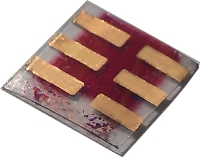
\includegraphics[width=30mm]{./images/cell.jpg}
%\label{overflow}
%\end{figure}

\newpage

\ClearWallPaper

\vspace*{\fill}
Please do not cite this manual.  Please see the section \ref{sec:using_gvpdm} on how to cite the model in your work.
\vspace*{\fill}


Front cover: A picture of a thermal power station in \href{https://en.wikipedia.org/wiki/Ratcliffe-on-Soar_Power_Station}{Ratcliffe-on-Soar} Nottinghamshire taken on a cold January afternoon in 2017. Most of the emissions you see in the image is water from the cooling towers however the gasses rising form the tall thin chimney on the left hand side of the image are the products of burning hydrocarbons which previously buried in the ground for about 300 million years.
